\chapter{Data Emulators}
As can be seen from the growth-geometry split analysis, a great amount of time and computing resources are needed to do a comprehensive analysis of novel cosmological models and extensions to $\Lambda$CDM. There are a growing number of proposed extension theories, and more data sets that can test them. One of the ways to improve the efficiency of data and theory analysis is to create a faster way to compute data vectors when doing MCMC sampling. In this chapter, I will describe how one can use neural networks (NN) to learn this mapping, bypassing the need for expensive programs such as Comsolike.
\section{Neural Networks}
Although the term `neural network' is almost synonymous with magic in the modern world, the concept is very natural from elementary mathematics. We start with the most basic example: linear regression. 

In linear regression, one considers a model of the form $y=mx+b$. The goal is to find the values of $m$ and $b$ that minimizes the square of the residual
\begin{equation}
	L(y_{i,\mathrm{truth}},y_{i,\mathrm{model}}) = (y_{i,\mathrm{truth}} - y_{i,\mathrm{model}})^2\,.
\end{equation}
In this very special case, there is an analytic way to minimize $L$, but in general that is highly non-trivial. Additionally, there are much more complicated data sets one would want to model, such as data vectors in cosmological surveys. The remaining question is: how does one intelligently generalize this type of model to more complicated ones?

We have a tool that can do this already: the brain~\cite{noauthor_what_nodate}! The brain is a large system of cells called neurons. Each neuron is connected to others by a synapse, and after accumulating a large enough electric charge, the neuron will activate, sending the electric signal to a connected neuron. 

Using this, lets try to construct a general model. We start with the neurons
\begin{figure}[th]
	\centering
	\begin{tikzpicture}
		\draw (-2,0) circle (5pt);
		\draw (0,0) circle (5pt);
		\draw (2,0) circle (5pt);
		\draw (1,1.41) circle (5pt);
		\draw (-1,1.41) circle (5pt);
		\draw (1,-1.41) circle (5pt);
		\draw (-1,-1.41) circle (5pt);
	\end{tikzpicture}
	\caption{Arrangement of neurons.}
	\label{fig:neurons}
\end{figure}
Now we add in the synapses, the connections between neurons. In general, not every neuron is connected to each other. It should be noted, along each synapse is an activation function. Rather than having a threshold potential like a real synapse, NNs use functions that represent the activation of the neuron. Also, each synapse has a weight that represents the strength of the connection.
\begin{figure}[th]
	\centering
	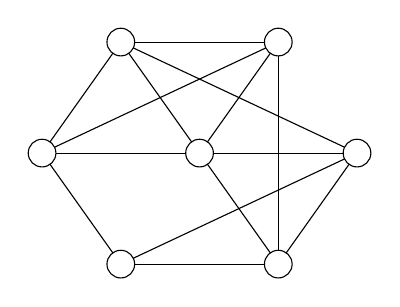
\begin{tikzpicture}
		\draw (-2,0) -- (0,0);
		\draw (-1,1.41) -- (0,0);
		\draw (-1,1.41) -- (-2,0);
		\draw (-1,-1.41) -- (-2,0);
		\draw (-1,-1.41) -- (1,-1.41);
		\draw (2,0) -- (1,-1.41);
		\draw (1,1.41) -- (-1,1.41);
		\draw (1,1.41) -- (1,-1.41);
		\draw (2,0) -- (-1,-1.41);
		\draw (0,0) -- (1,-1.41);
		\draw (0,0) -- (1,1.41);
		\draw (0,0) -- (2,0);
		\draw (-1,1.41) -- (2,0);
		\draw (1,1.41) -- (-2,0);
		\draw[fill=white] (-2,0) circle (5pt);
		\draw[fill=white] (0,0) circle (5pt);
		\draw[fill=white] (2,0) circle (5pt);
		\draw[fill=white] (1,1.41) circle (5pt);
		\draw[fill=white] (-1,1.41) circle (5pt);
		\draw[fill=white] (1,-1.41) circle (5pt);
		\draw[fill=white] (-1,-1.41) circle (5pt);
	\end{tikzpicture}
	\caption{Neurons with synapses.}
	\label{fig:neurons_synapse}
\end{figure}
Next, we define which neurons receive an external signal, and which give a signal to the outside. These act as our input and output.
\begin{figure}[th]
	\centering
	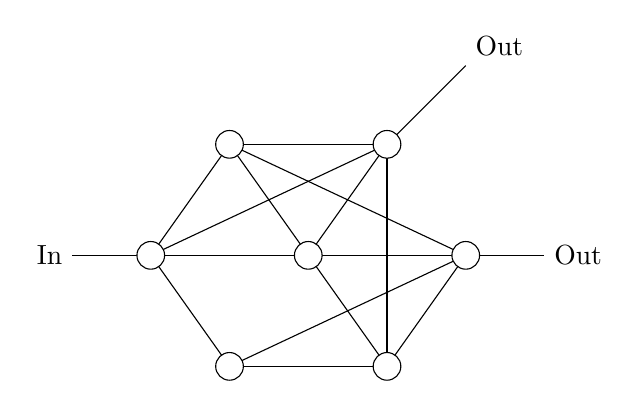
\begin{tikzpicture}
		\draw (-2,0) -- (0,0);
		\draw (-1,1.41) -- (0,0);
		\draw (-1,1.41) -- (-2,0);
		\draw (-1,-1.41) -- (-2,0);
		\draw (-1,-1.41) -- (1,-1.41);
		\draw (2,0) -- (1,-1.41);
		\draw (1,1.41) -- (-1,1.41);
		\draw (1,1.41) -- (1,-1.41);
		\draw (2,0) -- (-1,-1.41);
		\draw (0,0) -- (1,-1.41);
		\draw (0,0) -- (1,1.41);
		\draw (0,0) -- (2,0);
		\draw (-1,1.41) -- (2,0);
		\draw (1,1.41) -- (-2,0);
		\draw (-3,0) -- (-2,0);
		\draw (-3,0) node[anchor=east] {In};
		\draw (1,1.41) -- (2,2.41);
		\draw (2,0) -- (3,0);
		\draw (3,0) node[anchor=west] {Out};
		\draw (2,2.41) node[anchor=south west] {Out};
		\draw[fill=white] (-2,0) circle (5pt);
		\draw[fill=white] (0,0) circle (5pt);
		\draw[fill=white] (2,0) circle (5pt);
		\draw[fill=white] (1,1.41) circle (5pt);
		\draw[fill=white] (-1,1.41) circle (5pt);
		\draw[fill=white] (1,-1.41) circle (5pt);
		\draw[fill=white] (-1,-1.41) circle (5pt);
	\end{tikzpicture}
	\caption{Neurons, synapses, and IO.}
	\label{fig:neurons_synapse_io}
\end{figure}
Finally, we have a choice to make in the activation function. This is the chance to greatly increase the modelling capability of NNs. As we will see in the future, the only requirement is that the function is continuous, thus we can use non-linear activation functions, allowing modelling of highly non-linear outputs. The goal is to define a loss function function that we want to minimize (in the linear regression, the loss is the square of the residual). The loss function is a function of the output of the NN, and the output is parameterized by the parameters of the NN. Thus, if $y=\phi(\alpha_i,x)$ represents the output of the neural network with parameters $\alpha_i$ and input $x$, the loss function is, in fact, parameterized by the neural network as well.
\begin{equation}
	L(y) = L(\phi(\alpha_i,x)) = \mathfrak{L}(\alpha_i,x)
\end{equation}
Thus, a neural network is, in simple terms, an optimization problem. The issue, however, is that neural networks generally have a large number of parameters (thousands, millions, even billions!), so this optimization is difficult in practice. Also, what may appear as a simple loss function in terms of the output can become an extremely complicated (and importantly, non-monotonic) function of $\alpha_i$.

The general method of optimization is called \textit{gradient descent}. The strategy is the following:
\begin{enumerate}
	\item Define an initial set of parameters $\alpha_{i,\mathrm{init}}$.
	\item Split the training data into $n$ batches
	\item Generate a new set of parameters for each batch, centered around $\alpha_{i,\mathrm{init}}$, denoted $\alpha^{n}_{i}$.
	\item Compute the loss for each batch.
	\item Compute the gradient of the neural network.
	\item Update the parameters according to the gradient.
	\item Repeat until gradient is 0.
\end{enumerate}
This simple algorithm has one glaring flaw, it is prone to getting stuck in local minima. Ideally, we want to search for the global minimum for the loss function. The way around this is to add some stochasticity to the gradient descent so that the network does not simply search for zero gradient. Instead, the parameters are updated probabilistically from the gradient.

The gradient is usually computed using \textit{backpropagation}, in which the gradient is computed at each layer and the total gradient is computed according to the chain rule. This presents an issue: if the gradient is small at each layer, the gradient will be small on the order of $\epsilon^{n}$, where $n$ is the number of layers. This can lead to a misleading gradient that vanishes, or a gradient that explodes to large values. This is the problem of \textit{vanishing gradients}, and we will discuss ways to avoid this in the next section.

The last issue to mention is that, given a large number of parameters, its possible to fit the training data very well, but the model is not able to fit external data sets. This is called \textit{overfitting}. There are many strategies to resolve this. The two we will use is dropout and L2 regularization. Dropout randomly sets a fraction of the weights to zero, meaning the NN will not be able to rely on individual neurons to get a reliable output. This ensures the full network is being used. L2 regularization penalizes the model for learning large weights, which again means the model relies on particular neurons. This is accomplished by modifying the loss function by adding the L2 norm of the network.
\begin{equation}
	L(y) \mapsto L(y)+\sum_i \alpha_i^2
\end{equation}
In summary, a NN is a directed graph, where each edge has a weight and an activation function, and each node has a value that it passes along to the edge. The inputs are propagated to the output, and the goal is to minimize the loss of the output. Its important to pick a smart loss function depending on ones needs from the NN and a smart activation function depending on the values of each node. The loss function is minimized using stochastic gradient descent. It is important to also implement strategies to avoid overfitting on the training data by penalizing the model for relying to heavily on certain regions of the graph.
\section{Architecture Choices}
As discussed before, the weights, activation functions, and connections are choices we can make for a neural network. Together, they comprise the architecture. In this section we will discuss the architecture choices we have made.

Before discussing the graph architecture, we want to highlight the choice of activation function. Before giving any data to the neural network, we do some preprocessing to the data. The first thing we do is normalize the input and output. The input is the cosmological parameters, which we process each parameter to follow a normal distribution.
\begin{equation}
	x^i = \frac{\theta^i - \bar\theta^i}{\sigma_i}
\end{equation}
The output is the cosmic shear data vector. We prepreocess this by diagonalizing and normalizing each component.
\begin{equation}
	y^i = \frac{ (P^{-1}d)^i }{\sqrt{(PCP^{-1})^{ii}}}
\end{equation}
Where $C$ is the covariance of the data and $P$ the change of basis matrix to the eigenbasis of $C$. This generally means we will have a lot of negative parameters, and the input and output are both symmetric about 0, thus we choose to use an antisymmetric activation function so that the symmetry around 0 can be preserved. In our case, we use $\tanh(x)$. Additionally, all of these NNs are feedforward sequential models. Sequential means we separate the neurons into layers, and feedforward means the data moves only from layer $n$ to layer $n+1$ and never backwards.
\subsection{Multi-Layer Perceptron}
The first graph architecture we study in the multi-layer perceptron (the name is adopted from convolutional neural networks `perceiving' image features). In this architecture a node in a given layer is connected to every node in the following layer, so this network is called `simply connected' (figure~\ref{fig:mlp}).
\begin{figure}[ht]
	\centering
	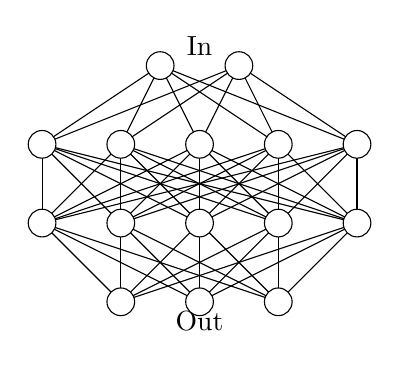
\begin{tikzpicture}
		\draw (0,2) node[anchor=south] {In};
		\draw (-0.5,2) -- (-2,1);
		\draw (-0.5,2) -- (-1,1);
		\draw (-0.5,2) -- (0,1);
		\draw (-0.5,2) -- (1,1);
		\draw (-0.5,2) -- (2,1);
		\draw (0.5,2) -- (-2,1);
		\draw (0.5,2) -- (-1,1);
		\draw (0.5,2) -- (0,1);
		\draw (0.5,2) -- (1,1);
		\draw (0.5,2) -- (2,1);
		%1-2
		\draw (-2,1) -- (-2,0);
		\draw (-2,1) -- (-1,0);
		\draw (-2,1) -- (0,0);
		\draw (-2,1) -- (1,0);
		\draw (-2,1) -- (2,0);
		\draw (-1,1) -- (-2,0);
		\draw (-1,1) -- (-1,0);
		\draw (-1,1) -- (0,0);
		\draw (-1,1) -- (1,0);
		\draw (-1,1) -- (2,0);
		\draw (0,1) -- (-2,0);
		\draw (0,1) -- (-1,0);
		\draw (0,1) -- (0,0);
		\draw (0,1) -- (1,0);
		\draw (0,1) -- (2,0);
		\draw (1,1) -- (-2,0);
		\draw (1,1) -- (-1,0);
		\draw (1,1) -- (0,0);
		\draw (1,1) -- (1,0);
		\draw (1,1) -- (2,0);
		\draw (2,1) -- (-2,0);
		\draw (2,1) -- (-1,0);
		\draw (2,1) -- (0,0);
		\draw (2,1) -- (1,0);
		\draw (2,1) -- (2,0);
		%2-3
		\draw (-2,0) -- (-1,-1);
		\draw (-2,0) -- (0,-1);
		\draw (-2,0) -- (1,-1);
		\draw (-1,0) -- (-1,-1);
		\draw (-1,0) -- (0,-1);
		\draw (-1,0) -- (1,-1);
		\draw (0,0) -- (-1,-1);
		\draw (0,0) -- (0,-1);
		\draw (0,0) -- (1,-1);
		\draw (1,0) -- (-1,-1);
		\draw (1,0) -- (0,-1);
		\draw (1,0) -- (1,-1);
		\draw (2,0) -- (-1,-1);
		\draw (2,0) -- (0,-1);
		\draw (2,0) -- (1,-1);
		\draw (0,-1) node[anchor=north] {Out};
		%layer in to 1
		\draw[fill=white] (-0.5,2) circle (5pt);
		\draw[fill=white] (0.5,2) circle (5pt);
		\draw[fill=white] (-2,1) circle (5pt);
		\draw[fill=white] (-1,1) circle (5pt);
		\draw[fill=white] (0,1) circle (5pt);
		\draw[fill=white] (1,1) circle (5pt);
		\draw[fill=white] (2,1) circle (5pt);
		\draw[fill=white] (-2,0) circle (5pt);
		\draw[fill=white] (-1,0) circle (5pt);
		\draw[fill=white] (0,0) circle (5pt);
		\draw[fill=white] (1,0) circle (5pt);
		\draw[fill=white] (2,0) circle (5pt);
		\draw[fill=white] (-1,-1) circle (5pt);
		\draw[fill=white] (0,-1) circle (5pt);
		\draw[fill=white] (1,-1) circle (5pt);
	\end{tikzpicture}
	\caption{A multi-layer perceptron.}
	\label{fig:mlp}
\end{figure}
\subsection{Residual Network}
As mentioned above, there is an issue of vanishing gradients with deep neural networks. To resolve this, one can add the input and output together so that gradient information is allowed to skip layers~\cite{he_deep_2015}(figure~\ref{fig:resblock}). Suppose we have a block of layers parameterized by $\alpha_i$, and its input is from another layer parameterized by $\beta_i$ so that $w=\chi(\beta_i,x)$ for an input $x$. Then the block of layers, whose map is denoted $\phi$, will be
\begin{equation}
	\phi(\alpha_i,\chi(\beta_i,x)) = \psi(\alpha_i,\beta_i,x)+\chi(\beta_i,x)
\end{equation}
This section of the model is going to attempt to learn
\begin{equation}
	\psi(\alpha_i,\beta_i,x)-\chi(\beta_i,x)
\end{equation}
This allows gradients with respect to the parameters $\beta_i$ to propagate to the output without the multiplication by the gradients of $\alpha_i$, which usually solves the vanishing gradient problem. This is called a \textit{residual neural network} (ResNet).
\begin{figure}[ht]
	\centering
	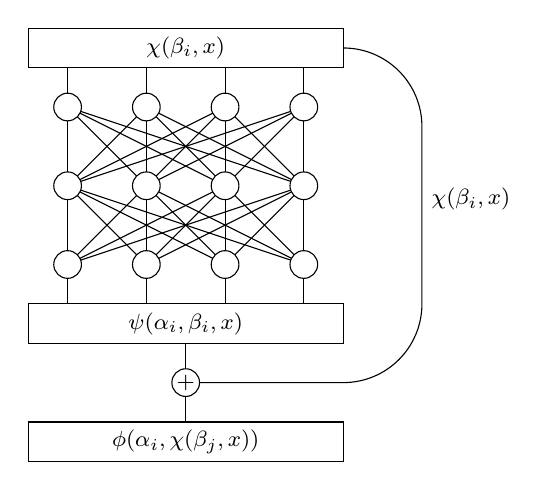
\begin{tikzpicture}
		\draw (0,2.75) node {\footnotesize $\chi(\beta_i,x)$};
		\draw (-2,2.5) -- (2,2.5) -- (2,3) -- (-2,3) -- (-2,2.5);
		\draw (-1.5,2.5) -- (-1.5,2);
		\draw (-0.5,2.5) -- (-0.5,2);
		\draw (0.5,2.5) -- (0.5,2);
		\draw (1.5,2.5) -- (1.5,2);
		%in
		\draw (-1.5,2) -- (-1.5,1);
		\draw (-1.5,2) -- (-0.5,1);
		\draw (-1.5,2) -- (0.5,1);
		\draw (-1.5,2) -- (1.5,1);
		\draw (-0.5,2) -- (-1.5,1);
		\draw (-0.5,2) -- (-0.5,1);
		\draw (-0.5,2) -- (0.5,1);
		\draw (-0.5,2) -- (1.5,1);
		\draw (0.5,2) -- (-1.5,1);
		\draw (0.5,2) -- (-0.5,1);
		\draw (0.5,2) -- (0.5,1);
		\draw (0.5,2) -- (1.5,1);
		\draw (1.5,2) -- (-1.5,1);
		\draw (1.5,2) -- (-0.5,1);
		\draw (1.5,2) -- (0.5,1);
		\draw (1.5,2) -- (1.5,1);
		%%% hidden
		\draw (-1.5,1) -- (-1.5,0);
		\draw (-1.5,1) -- (-0.5,0);
		\draw (-1.5,1) -- (0.5,0);
		\draw (-1.5,1) -- (1.5,0);
		\draw (-0.5,1) -- (-1.5,0);
		\draw (-0.5,1) -- (-0.5,0);
		\draw (-0.5,1) -- (0.5,0);
		\draw (-0.5,1) -- (1.5,0);
		\draw (0.5,1) -- (-1.5,0);
		\draw (0.5,1) -- (-0.5,0);
		\draw (0.5,1) -- (0.5,0);
		\draw (0.5,1) -- (1.5,0);
		\draw (1.5,1) -- (-1.5,0);
		\draw (1.5,1) -- (-0.5,0);
		\draw (1.5,1) -- (0.5,0);
		\draw (1.5,1) -- (1.5,0);
		%%%
		\draw (-1.5,-0.5) -- (-1.5,0);
		\draw (-0.5,-0.5) -- (-0.5,0);
		\draw (0.5,-0.5) -- (0.5,0);
		\draw (1.5,-0.5) -- (1.5,0);
		%%%
		\draw (-2,-0.5) -- (2,-0.5) -- (2,-1) -- (-2,-1) -- (-2,-0.5);
		\draw (-2,-2) -- (2,-2) -- (2,-2.5) -- (-2,-2.5) -- (-2,-2);
		\draw (0,-0.75) node {\footnotesize $\psi(\alpha_i,\beta_i,x)$};
		\draw (0,-1) -- (0,-2);
		\draw (2,2.75) to[out=0,in=90] (3,1.75) -- (3,-0.5) to[out=-90,in=0] (2,-1.5) -- (0,-1.5);
		\draw (0,-2.25) node {\footnotesize $\phi(\alpha_i,\chi(\beta_j,x))$};
		\draw (3,0.83) node[anchor=west] {\footnotesize $\chi(\beta_i,x)$};
		%layer in to 1
		\draw[fill=white] (-1.5,2) circle (5pt);
		\draw[fill=white] (-0.5,2) circle (5pt);
		\draw[fill=white] (0.5,2) circle (5pt);
		\draw[fill=white] (1.5,2) circle (5pt);
		\draw[fill=white] (-1.5,1) circle (5pt);
		\draw[fill=white] (-0.5,1) circle (5pt);
		\draw[fill=white] (0.5,1) circle (5pt);
		\draw[fill=white] (1.5,1) circle (5pt);
		\draw[fill=white] (-1.5,0) circle (5pt);
		\draw[fill=white] (-0.5,0) circle (5pt);
		\draw[fill=white] (0.5,0) circle (5pt);
		\draw[fill=white] (1.5,0) circle (5pt);
		\draw[fill=white] (0,-1.5) circle (5pt);
		\draw (0,-1.5) node {\footnotesize{$+$}};
	\end{tikzpicture}
	\caption{A residual block.}
	\label{fig:resblock}
\end{figure}
\subsection{Bottlenecked Residual Network}
The ResNet allows us to create much deeper networks, but the number of parameters stays the same as the linear model, making ResNets difficult to train (and especially the minimum of two linear layers. We can make a small modification to the ResNet that can resolve this, where there is an additional layer and the number of dimensions reduces in the middle (figure~\ref{fig:resbottle-block}). This forces the neural network to prioritize certain features and ignore ones that are not as necessary. Due to the shape this architecture makes, its referred to as a \textit{bottlenecked residual network} (ResBottle) (figure~\ref{fig:resbottle-block}).
\begin{figure}[ht]
	\centering
	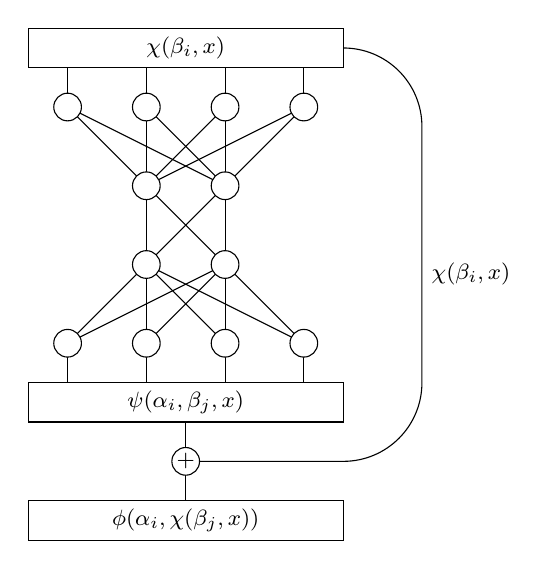
\begin{tikzpicture}
		\draw (1.5,1) -- (0.5,0);
		\draw (1.5,1) -- (-0.5,0);
		\draw (0.5,1) -- (0.5,0);
		\draw (0.5,1) -- (-0.5,0);
		\draw (-0.5,1) -- (0.5,0);
		\draw (-0.5,1) -- (-0.5,0);
		\draw (-1.5,1) -- (0.5,0);
		\draw (-1.5,1) -- (-0.5,0);
		\draw (-0.5,0) -- (-0.5,-1);
		\draw (-0.5,0) -- (0.5,-1);
		\draw (0.5,0) -- (-0.5,-1);
		\draw (0.5,0) -- (0.5,-1);
		\draw (1.5,-2) -- (0.5,-1);
		\draw (1.5,-2) -- (-0.5,-1);
		\draw (0.5,-2) -- (0.5,-1);
		\draw (0.5,-2) -- (-0.5,-1);
		\draw (-0.5,-2) -- (0.5,-1);
		\draw (-0.5,-2) -- (-0.5,-1);
		\draw (-1.5,-2) -- (0.5,-1);
		\draw (-1.5,-2) -- (-0.5,-1);
		%%%
		\draw (-1.5,1.5) -- (-1.5,1);
		\draw (-0.5,1.5) -- (-0.5,1);
		\draw (0.5,1.5) -- (0.5,1);
		\draw (1.5,1.5) -- (1.5,1);
		\draw (-1.5,-2.5) -- (-1.5,-2);
		\draw (-0.5,-2.5) -- (-0.5,-2);
		\draw (0.5,-2.5) -- (0.5,-2);
		\draw (1.5,-2.5) -- (1.5,-2);
		\draw (-2,-2.5) -- (2,-2.5) -- (2,-3) -- (-2,-3) -- (-2,-2.5);
		\draw (-2,1.5) -- (2,1.5) -- (2,2) -- (-2,2) -- (-2,1.5);
		%%%
		\draw (0,-4) -- (0,-3);
		\draw (-2,-4.5) -- (2,-4.5) -- (2,-4) -- (-2,-4) -- (-2,-4.5);
		%%%
		\draw[fill=white] (1.5,1) circle (5pt);
		\draw[fill=white] (0.5,1) circle (5pt);
		\draw[fill=white] (-0.5,1) circle (5pt);
		\draw[fill=white] (-1.5,1) circle (5pt);
		%%%
		\draw[fill=white] (0.5,0) circle (5pt);
		\draw[fill=white] (-0.5,0) circle (5pt);
		%%%
		\draw[fill=white] (0.5,-1) circle (5pt);
		\draw[fill=white] (-0.5,-1) circle (5pt);
		%%%
		\draw[fill=white] (1.5,-2) circle (5pt);
		\draw[fill=white] (0.5,-2) circle (5pt);
		\draw[fill=white] (-0.5,-2) circle (5pt);
		\draw[fill=white] (-1.5,-2) circle (5pt);
		%%%
		\draw (2,1.75) to[out=0,in=90] (3,0.75) -- (3,-2.5) to[out=-90,in=0] (2,-3.5) -- (0,-3.5);
		\draw[fill=white] (0,-3.5) circle (5pt);
		\draw (0,-3.5) node {\footnotesize $+$};
		\draw (0,1.75) node {\footnotesize $\chi(\beta_i,x)$};
		\draw (0,-2.75) node {\footnotesize $\psi(\alpha_i,\beta_j,x)$};
		\draw (0,-4.25) node {\footnotesize $\phi(\alpha_i, \chi(\beta_j,x))$};
		\draw (3,-1.12) node[anchor=west] {\footnotesize $\chi(\beta_i,x)$};
	\end{tikzpicture}
	\caption{A bottlenecked residual block.}
	\label{fig:resbottle-block}
\end{figure}
In the examples drawn (figures~\ref{fig:resblock} and~\ref{fig:resbottle-block}), there are 40 parameters in the ResNet, but only 28 parameters in the ResBottle. This allows us to either simplify the model, add more layers, or make the layers much wider without blowing up the number of parameters that need to be trained.
\subsection{Attention}
This will be the most complicated model to test. If we look at the structure of the data vector, there is a certain order to the data and correlation between the components. The data vectors is separated into redshift bins, and within each redshift bin are bins representing different scales. Thus, a NN that can learn sequences may be useful. Fortunately, there are NNs we encounter everyday that use sequences: chatbots! The basis for this is usually attention networks~\cite{vaswani_attention_2017}. These work by examining dot products between vectors so that the output is directly related to the angle between the two vectors.

suppose we are given a sequence of input vectors, $x=(x_1,x_2,\ldots,x_n)$, then we can construct dot products of the $x_i$ and use them as coefficients for the output.
\begin{equation}
	y_k = (x_i \cdot x_j)x_k
\end{equation}
We can introduce generalize the dot product using linear transformations. That is, we can introduce the transformation matrices $W_Q$, $W_K$, $W_V$. Let $q_i = W_Q x_i$, $k_i = W_K x_i$, and $v_i = W_V x_i$. Then we can also write a dot product as 
\begin{equation}
	y_k = (q_i^T k_j)v_k
\end{equation}
Finally, we can introduce a non-linearity, which also keeps the outputs sequence $y$ normalized. By introducing the \textit{softmax} function.
\begin{equation}
	y_k = \mathrm{softmax}(q_i^T k_j / \sqrt{d})v_k
\end{equation}
where the softmax function is an exponential normalization given by
\begin{equation}
	\mathrm{softmax}(W)_i = \frac{e^{w_i}}{e^{\sum_i{w_i}}}
\end{equation}
and $d$ is the embedding dimension (i.e $W_K\in \mathbb{R}^{d_x\times d}$).
We allow the linear matrices $W_Q$, $W_K$, and $W_V$ to contain learnable components. We then pass each output $y_i$ to its own MLP. We also keep the skip connections describe in the residual network section. The attention together with the MLPs and skip connections is called a transformer block, drawn in figure~\ref{fig:attention}.
\begin{figure}[ht]
	\centering
	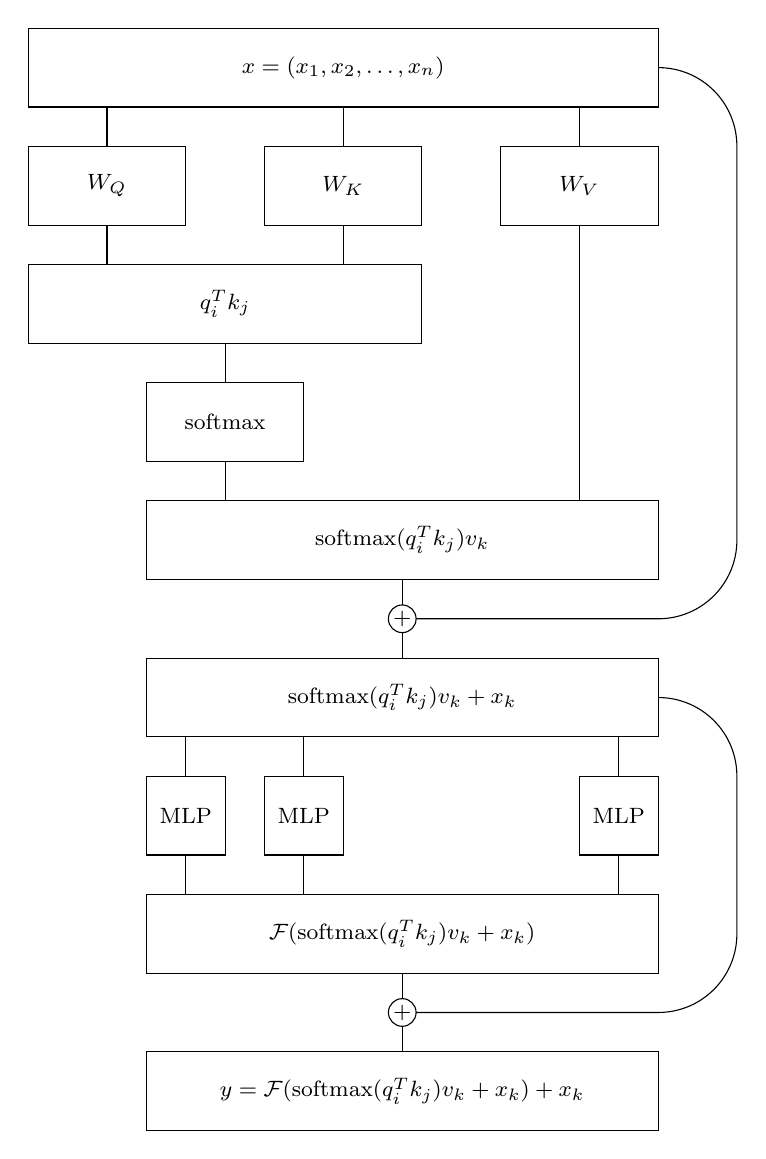
\begin{tikzpicture}
		%%curved skip lines
		\draw (8,2.5) to[out=0,in=90] (9,1.5) -- (9,-3.5) to[out=-90,in=0] (8,-4.5) -- (4.75,-4.5);
		\draw (8,-5.5) to[out=0,in=90] (9,-6.5) -- (9,-8.5) to[out=-90,in=0] (8,-9.5) -- (4.75,-9.5);
		%%input
		\draw (0,2) -- (8,2) -- (8,3) -- (0,3) -- (0,2);
		\draw (4,2.5) node {\footnotesize $x=(x_1,x_2,\dots,x_n)$};
		%%next!
		%\draw (1,4) node[anchor=south] {\footnotesize $x_i$};
		\draw (1,2) -- (1,1.5);
		\draw (1,1) node {\footnotesize $W_Q$};
		\draw (0,1.5) -- (0,0.5) -- (2,0.5) -- (2,1.5) -- (0,1.5);
		%\draw (4,4) node[anchor=south] {\footnotesize $x_j$};
		\draw (4,2) -- (4,1.5);
		\draw (4,1) node {\footnotesize $W_K$};
		\draw (3,1.5) -- (3,0.5) -- (5,0.5) -- (5,1.5) -- (3,1.5);
		%%next!
		\draw (1,0.5) -- (1,0);
		\draw (4,0.5) -- (4,0);
		\draw (5,-1) -- (0,-1) -- (0,0) -- (5,0) --  (5,-1);
		\draw (2.5,-0.5) node {\footnotesize $q_i^T k_j$};
		%%next!
		%\draw (7,4) node[anchor=south] {\footnotesize $x_k$};
		\draw (7,2) -- (7,1.5);
		\draw (7,1) node {\footnotesize $W_V$};
		\draw (6,1.5) -- (6,0.5) -- (8,0.5) -- (8,1.5) -- (6,1.5);
		%%next!
		\draw (2.5,-1) -- (2.5,-1.5);
		\draw (1.5,-1.5) -- (1.5,-2.5) -- (3.5,-2.5) -- (3.5,-1.5) -- (1.5,-1.5);
		\draw (2.5,-2) node {\footnotesize softmax};
		%%next!
		\draw (7,0.5) -- (7,-3);
		\draw (2.5,-2.5) -- (2.5,-3);
		\draw (1.5,-3) -- (1.5,-4) -- (8,-4) -- (8,-3) -- (1.5,-3);
		\draw (4.75,-3.5) node {\footnotesize $\mathrm{softmax}(q_i^T k_j)v_k$};
		%%skips!
		\draw (4.75,-4) -- (4.75,-5);
		\draw[fill=white] (4.75,-4.5) circle (5pt);
		\draw (4.75,-4.5) node {\footnotesize $+$};
		%mlps
		\draw (1.5,-5) -- (1.5,-6) -- (8,-6) -- (8,-5) -- (1.5,-5);
		\draw (4.75,-5.5) node {\footnotesize $\mathrm{softmax}(q_i^T k_j)v_k + x_k$};
		\draw (2,-6) -- (2,-6.5);
		\draw (1.5,-6.5) -- (1.5,-7.5) -- (2.5,-7.5) -- (2.5,-6.5) -- (1.5,-6.5);
		\draw (2,-7) node {\footnotesize MLP};
		\draw (3.5,-6) -- (3.5,-6.5);
		\draw (3,-6.5) -- (3,-7.5) -- (4,-7.5) -- (4,-6.5) -- (3,-6.5);
		\draw (3.5,-7) node {\footnotesize MLP};
		\draw (5.5,-7) node {$\hdots$};
		\draw (7.5,-6) -- (7.5,-6.5);
		\draw (7,-6.5) -- (7,-7.5) -- (8,-7.5) -- (8,-6.5) -- (7,-6.5);
		\draw (7.5,-7) node {\footnotesize MLP};
		%%last skip
		\draw (7.5,-7.5) -- (7.5,-8);
		\draw (3.5,-7.5) -- (3.5,-8);
		\draw (2,-7.5) -- (2,-8);
		\draw (1.5,-8) -- (1.5,-9) -- (8,-9) -- (8,-8) -- (1.5,-8);
		\draw (4.75,-8.5) node {\footnotesize $\mathcal{F}(\mathrm{softmax}(q_i^T k_j)v_k + x_k)$};
		\draw (4.75,-9) -- (4.75,-10);
		\draw (1.5,-10) -- (1.5,-11) -- (8,-11) -- (8,-10) -- (1.5,-10);
		\draw[fill=white] (4.75,-9.5) circle (5pt);
		\draw (4.75,-9.5) node {\footnotesize $+$};
		\draw (4.75,-10.5) node {\footnotesize $y = \mathcal{F}(\mathrm{softmax}(q_i^T k_j)v_k + x_k)+x_k$};
	\end{tikzpicture}
	\caption{A transformer block}
	\label{fig:attention}
\end{figure}

\section{Results}
We present the results in two sections: the first will be about the training and testing results, and the second comparing between a cocoa chain and an emulated chain. For training and testing, we use the "train, validate, test" approach. We generate three completely independent chains, one is only for training the model, and is a high temperature chain with data well beyond the expected range. The second is used to validate that the model is not overfitting as the training proceeds. The last set is another high temperature chain (but not as high as the training) which is used to test the model as if it were being used as normal. The testing involves reintroducing specific analysis choices such as the scale cut.

When deciding on which model to use, we want to look at several aspects:
\begin{itemize}
	\item The number of parameters. The more parameters we have, the longer it takes to train, and the longer it takes to evaluate. This will make it difficult for groups without top-of-the-line equipment.
	\item The $\Delta\chi^2$ between the emulator and accepted computational methods. Many experiments have a $\chi^2$ requirement for their emulators; for example DES requires $\Delta\chi^2<0.3$ between any approximations and Cosmolike.
	\item Generalizability. As we increase the volume covered in the parameter space, which models are able to keep up with the growing modelling volume? Which models can handle more input parameters (which many models need, such as early dark energy with $\sim10$ extra parameters).
\end{itemize}
These get analyzed on the test data set. Because of the second point above, we define the loss function as the difference in $\chi^2$ between the emulator and cosmolike. This allows us to capture the covariances in the data.
\subsection{Training and Testing}
We train the emulator by using a rough Gaussian approximation on the cosmological parameters. The benefit is that running MCMC chains on a simple Gaussian without the need for cosmolike is extremely fast. Given the samples, the data vector calculation is trivially parallelizable, so the entire process is significantly faster than running an MCMC in cosmolike. 

First, we examine the training and validation loss at each epoch. The training loss is the average loss of all batches in an epoch. Figure~\ref{fig:train_loss_resnet} displays the training loss of a ResNet model with 3 ResNet blocks and 256 neurons in each hidden layer. In this case, we can see a consistent decline in both the training and validation loss. Additionally, we can see the points where the learning rate decreases (see epoch 50 and epoch 85 in figure~\ref{fig:train_loss_resnet}) which occur when validation loss plateaus, following the expected behaviour. This demonstrates that we are likely not overfitting the training data.
\begin{figure}[tb]
	\centering
	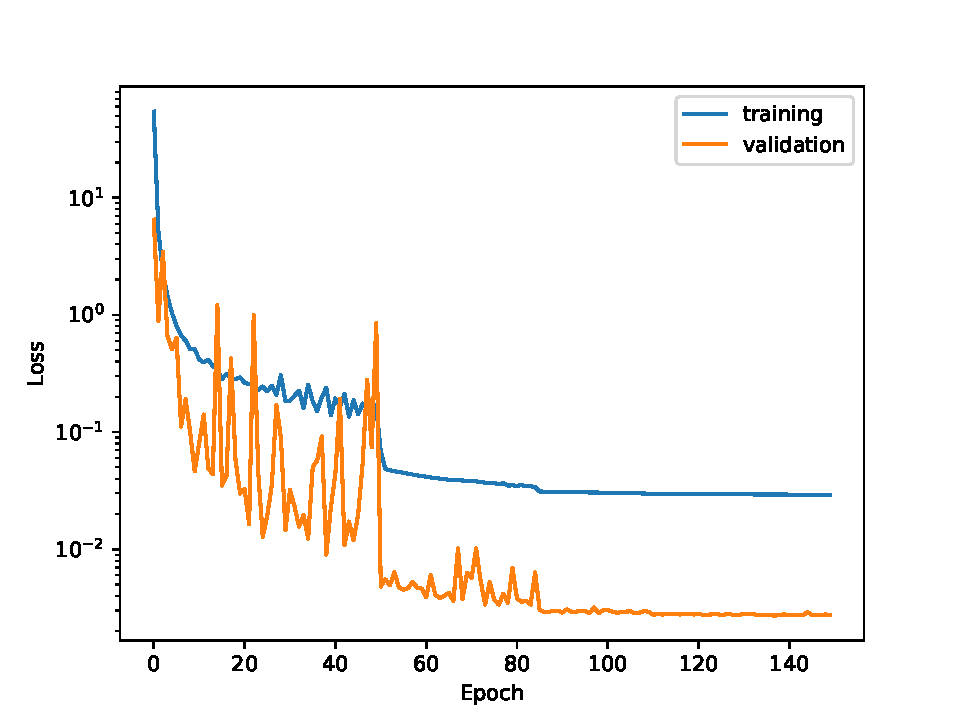
\includegraphics[width=0.9\textwidth]{plots/losses_resnet_3_256.pdf}
	\caption{Loss of a ResNet model with 3 ResNet blocks and 256 neurons in each layer.}
	\label{fig:train_loss_resnet}
\end{figure}
Using a trained model, we evaluate $\Delta\chi^2$ on the test data, a $T=8$ Gaussian approximated chain (figure~\ref{fig:testing_loss}). As we can see, our model is able to generalize well to a $T=8$ chain. 
\begin{figure}[tb]
	\centering
	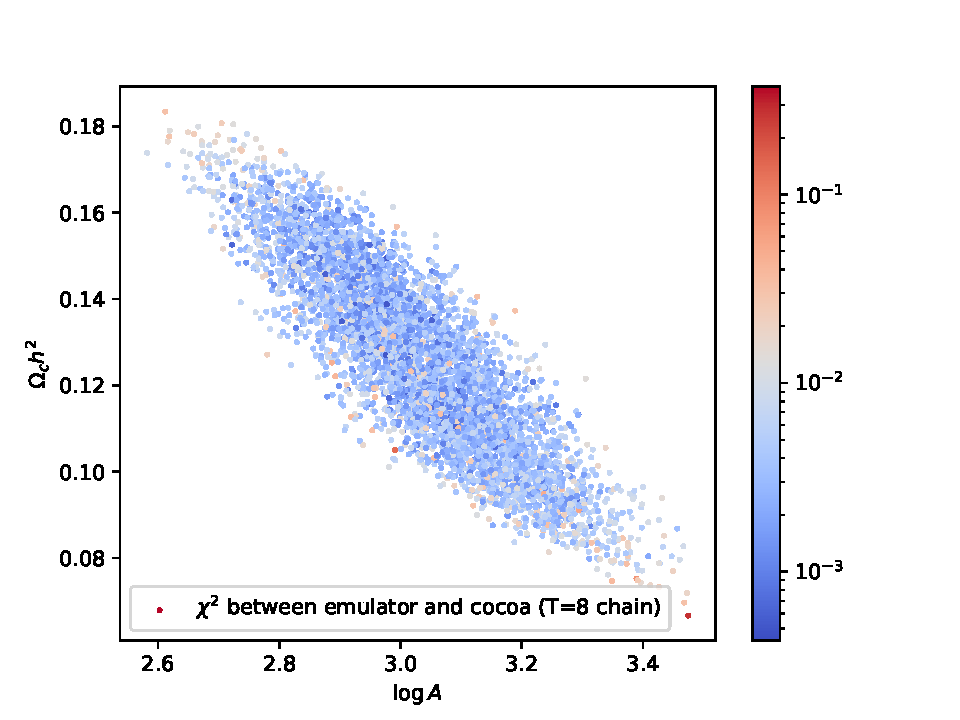
\includegraphics[width=0.9\textwidth]{plots/cosmic_shear_resnet_nlayer_3_intdim_256.pdf}
	\caption{Testing loss on a $T=8$ chain.}
	\label{fig:testing_loss}
\end{figure}

Additionally, we can test how high of a temperature we can train on and still get satisfactory performance.

\begin{figure}[tb]
	\centering
	\begin{subfigure}[b]{0.49\textwidth}
		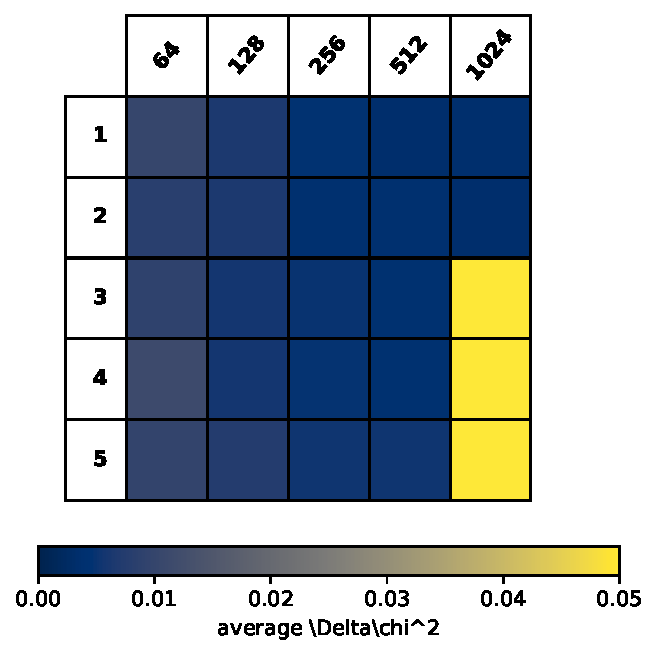
\includegraphics[width=\textwidth]{plots/model_table_mlp.pdf}
		\caption{MLP average loss}
		\label{fig:mlp_table}
	\end{subfigure}
	\begin{subfigure}[b]{0.49\textwidth}
		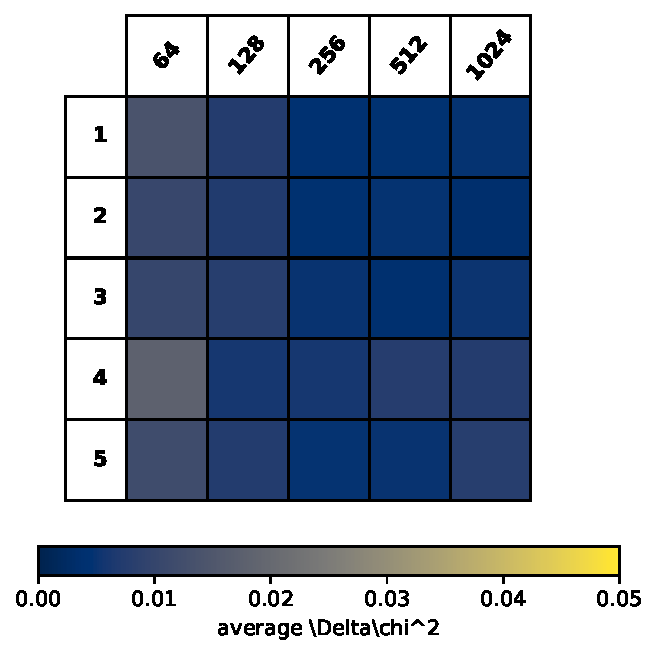
\includegraphics[width=\textwidth]{plots/model_table_resnet.pdf}
		\caption{ResNet average loss}
		\label{fig:resnet_table}
	\end{subfigure}
	\begin{subfigure}[b]{0.9\textwidth}
		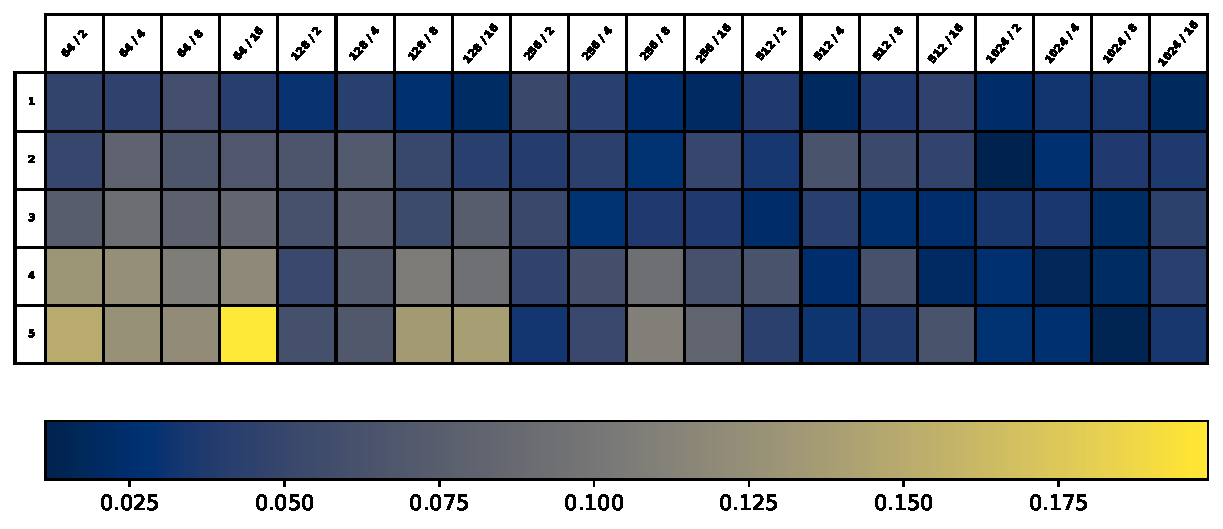
\includegraphics[width=\textwidth]{plots/model_table_resbottle.pdf}
		\caption{ResBottle average loss}
		\label{fig:resbottle_table}
	\end{subfigure}
	\label{fig:model_tables}
\end{figure}

\begin{figure}[tb]
	\centering
	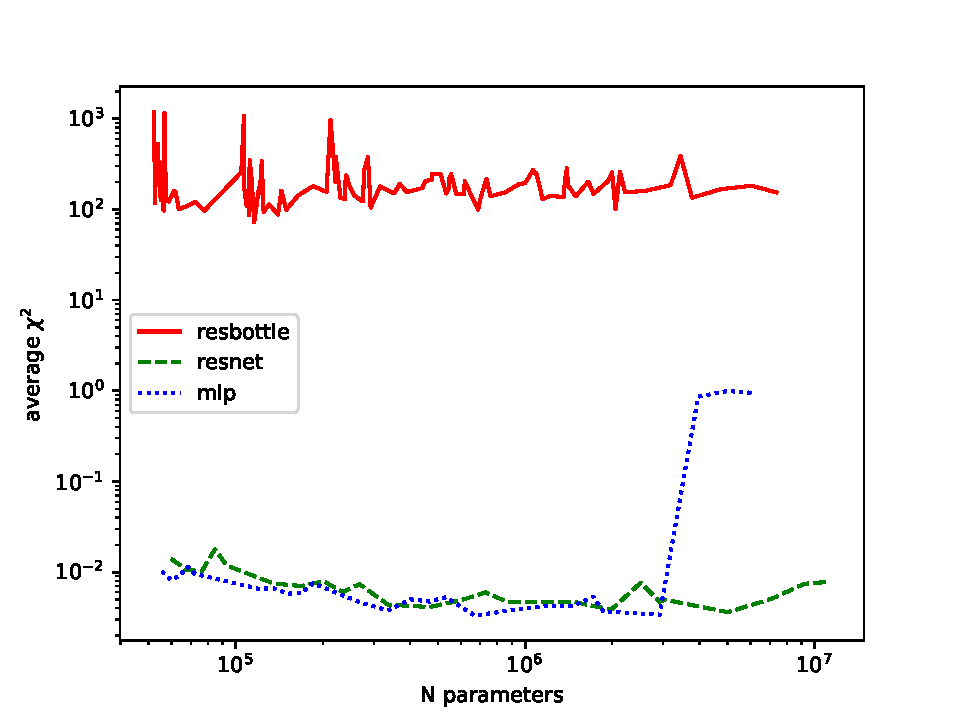
\includegraphics[width=0.9\textwidth]{plots/avg_chi2_v_n_params_new.pdf}
	\caption{Average $\chi^2$ as a function of the number of parameters for each architecture.}
	\label{fig:avg_chi2_nparams}
\end{figure}
\section{Application to Tension Calibration}
As mentioned in section~\ref{section}, tension metrics require calibration between experiments. In this section, I will apply the use of emulators to do a first study of tension metric error. By shifting the parameters and generating noise realizations on the data, we can get a sense of how the error in the data propagates to error in the tension. This will provide additional information as to which tension metrics perform best, as well as adding context to how tension may vary given new measurements. Additionally, given that $n_\sigma=0$ means no tension, the error are tension metrics will allow us to gauge how reasonable it may be for the tension to be resolved by additional identical measurements.

I will be shifting the LSST fiducial cosmology to $\pm5\sigma$ in both the $\sigma_8$ and $\Omega_m$ directions (figure~\ref{figure}). At each of these shifts, I will compute 1000 noise realizations on LSST cosmic shear using the data covariance. Finally, the tension will be computed using the methods described in section~\ref{section}.

I chose to use the ResNet model with 3 ResBlocks and $256$ neurons in each hidden layer. This model provides good stability in the predictions, and is sufficiently small that running chains on the noise realizations is tractable.









